\documentclass{beamer}

% \usepackage{beamerthemesplit} // Activate for custom appearance

\title{Nonparametric Regression and Bonferroni joint confidence intervals}
\author{Frank Wood}
%\date{\today}

\newcommand{\comment}[1]{}
\newcommand{\ponedec}{\mathcal{P}^\downarrow_1}
\newcommand{\pone}{\mathcal{P}_1}
\newcommand{\rank}[1]{\mathrm{RANK}\left[#1\right]}
\newcommand{\E}[1]{\mathrm{E}\left[#1\right]}
\newcommand{\py}{\mathcal{PY}}
\newcommand{\iid}{iid.}
\newcommand{\drawiid}{\stackrel{\text{iid}}{\sim}}
\newcommand{\vect}[1]{\mathbf{#1}}
\newcommand{\indicator}[1]{\text{I}\left[ #1 \right]}
\newcommand{\pdcoag}{PD(d_1,0)-\text{COAG}}
\newcommand{\todo}{\textbf{*TODO*}}
\newcommand{\igram}{\text{$\infty$-gram}}
\newcommand{\Prob}{\text{P}}

\def\mm{sequence memoizer }
\def\MM{SM }

\def\pibf{{\boldsymbol{\pi}}}
\def\kapbf{\boldsymbol{\kappa}}
\def\taubf{\boldsymbol{\tau}}
\def\thebf{\boldsymbol{\theta}}
\def\rhobf{\boldsymbol{\rho}}
\def\phibf{\boldsymbol{\phi}}
\def\pbf{\mathbf{p}}
\def\qbf{\mathbf{q}}
\def\sbf{\mathbf{s}}
\def\tbf{\mathbf{t}}
\def\ybf{\mathbf{y}}
\def\wbf{\mathbf{w}}
\def\xbf{\mathbf{x}}
\def\rbf{\mathbf{r}}
\def\tbf{\mathbf{t}}
\def\kbf{\mathbf{k}}
\def\Xbf{\mathbf{X}}
\def\0bf{\mathbf{0}}
\def\Ibf{\mathbf{I}}
\def\phibf{\mathbf{\phi}}
\def\Phibf{\mathbf{\Phi}}
\def\disteq{{\stackrel{D}{=}}}
\def\EE{{\mathbb{E}}}

\def\phiv{\varphi}
\def\phivbf{\boldsymbol{\varphi}}

\def\Ocal{\mathcal{O}}

\DeclareMathOperator*{\Bet}{Beta} \DeclareMathOperator{\coag}{COAG}
\DeclareMathOperator{\frag}{FRAG} \DeclareMathOperator*{\rnk}{RANK}
\DeclareMathOperator*{\gem}{GEM} \DeclareMathOperator*{\pd}{PD}
\DeclareMathOperator*{\gd}{GDir} \DeclareMathOperator*{\Dir}{Dir}
\DeclareMathOperator*{\Ave}{\mathbb{E}}
\DeclareMathOperator*{\Var}{Var}

\begin{document}

\frame{\titlepage}

%\section[Outline]{}
%\frame{\tableofcontents}
%
%\section{Introduction}
%\subsection{Overview of Topics}
%
%\section{Bayesian Analysis}
%\subsection{Single Parameter Model}
\frame[t] {
 \frametitle{Nonparametric Regression Curves}
 \begin{itemize}
\item So far: parametric regression approaches
\begin{itemize}
\item Linear
\item Linear with transformed inputs and outputs
\item etc.
\end{itemize}
\item Other approaches
\begin{itemize}
\item Method of moving averages : interpolate between mean outputs at adjacent inputs
\item Lowess : ``locally weighted scatterplot smoothing''
\end{itemize}
\end{itemize}

}

\frame[t] {
 \frametitle{Lowess Method}
 \begin{itemize}
\item Intuition
\begin{itemize}
\item Fit low-order polynomial (linear) regression models to points in a neighborhood
\begin{itemize}
\item The neighborhood size is a parameter
Determining the neighborhood is done via a nearest neighbors algorithm
\end{itemize}
Produce predictions by weighting the regressors by how far the set of points used to produce the regressor is from the input point for which a prediction is wanted
\end{itemize}
\item While somewhat ad-hoc, it is a method of producing a nonlinear regression function for data that might seem otherwise difficult to regress
\end{itemize}

}

\frame[t] {
 \frametitle{Lowess Method Example}
\begin{figure}[h!]
   \centering
    % \caption{}
     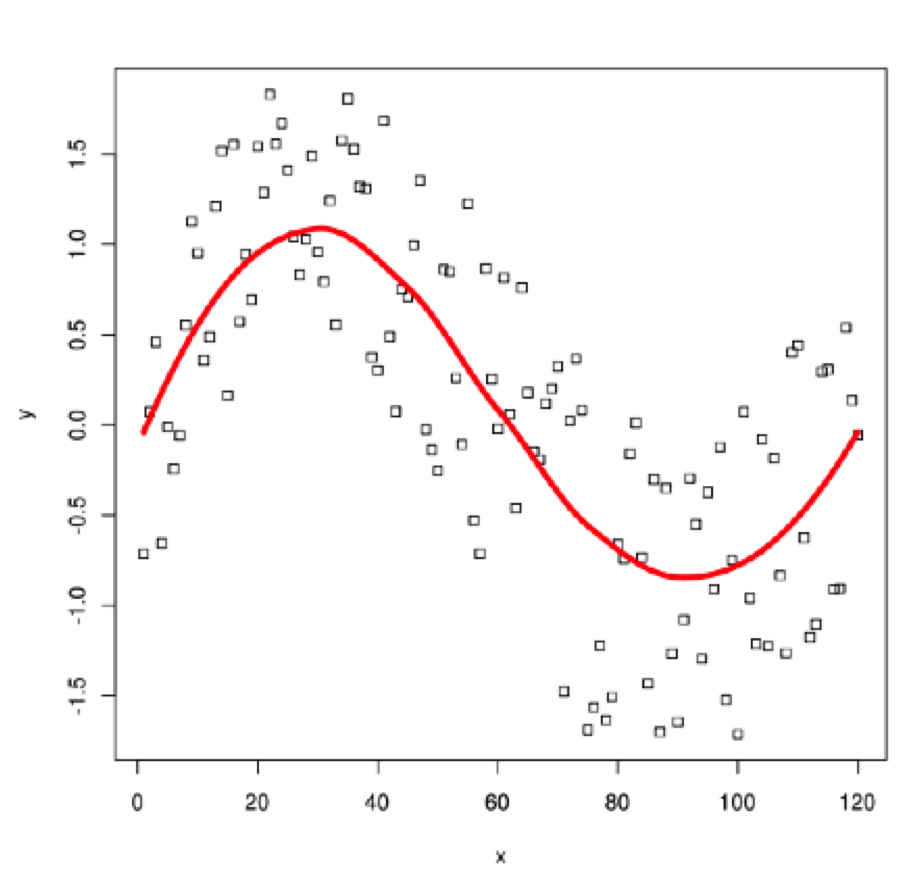
\includegraphics[scale=.5]{loess.png}
 \end{figure}

}

\frame[t] {
 \frametitle{Bonferroni Joint Confidence Intervals}
 \begin{itemize}
\item Calculation of Bonferroni joint confidence intervals is a general technique
\item We highlight its application in the regression setting
\begin{itemize}
\item Joint confidence intervals for $\beta_0$ and $\beta_1$
\end{itemize}
\item Intuition
\begin{itemize}
\item Set each statement confidence level to greater than $1-\alpha$ so that the family coefficient is at least $1-\alpha$
\end{itemize}
\end{itemize}

}

\frame[t] {
 \frametitle{Ordinary Confidence Intervals}
 \begin{itemize}
\item Start with ordinary confidence intervals for $\beta_0$ and $\beta_1$
\begin{eqnarray*}
b_0 \pm t(1-\alpha/2; n-2)s\{b_0\}\\
b_1 \pm t(1-\alpha/2; n-2)s\{b_1\}
\end{eqnarray*}
\item And ask what the probability that one or both of these intervals is incorrect
\end{itemize}

Remember 

\begin{eqnarray*}
s^2\{b_0\} &=& MSE\left[\frac{1}{n}+\frac{\bar X^2}{\sum(X_i-\bar X)^2}\right]\\
s^2\{b_1\} &=& \frac{MSE}{\sum(X_i-\bar X)^2}
\end{eqnarray*}

}

\frame[t] {
 \frametitle{General Procedure}
 \begin{itemize}
\item Let $A_1$ denote the event that the first confidence interval does not cover $\beta_0$, i.e.~$P(A_1) = \alpha$
\item Let $A_2$ denote the event that the second confidence interval does not cover $\beta_1$, i.e.~$P(A_2) = \alpha$
\item We want to know the probability that both estimates fall in their respective confidence intervals, i.e.~$P(\bar A_1 \cap \bar A_2)$
\item How do we get there from what we know?
\end{itemize}
}

\frame[t] {
 \frametitle{Venn Diagram}
\begin{figure}[h!]
   \centering
    % \caption{}
     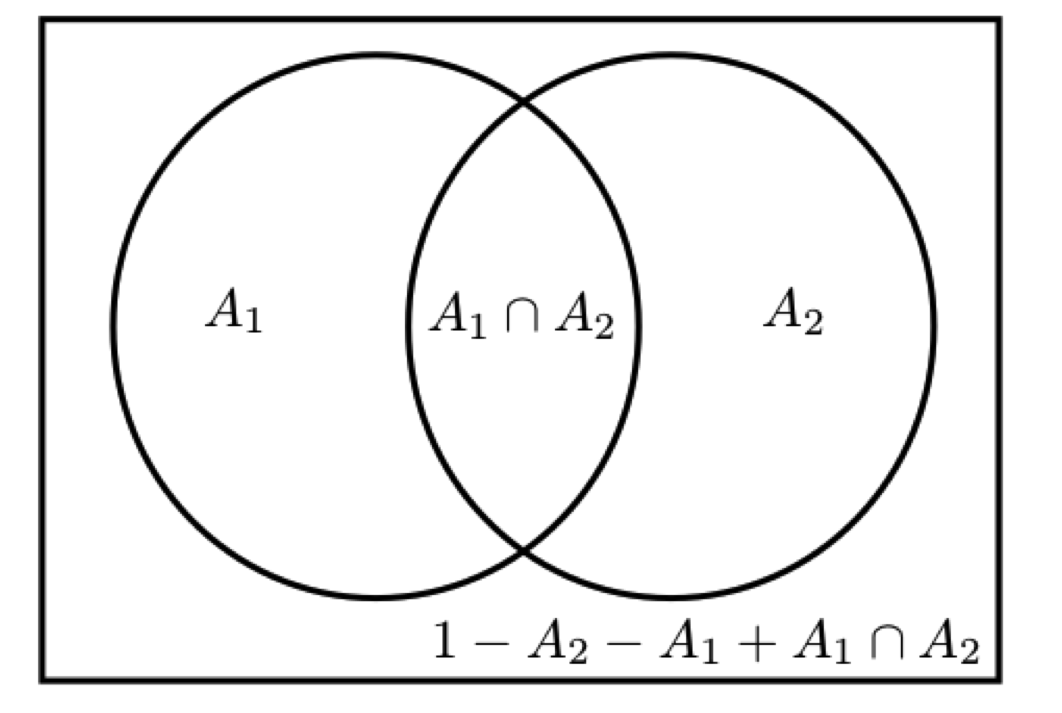
\includegraphics[scale=.5]{venn.png}
 \end{figure}

}

\frame[t] {
 \frametitle{Bonferroni inequality}
 \begin{itemize}
 \item We can see that $P(\bar A_1 \cap \bar A_2) = 1 - P(A_2) -P( A_1) + P(A_1 \cap A_2)$ 
 \begin{itemize}
\item Size of set is equal to area is equal to probability in a Venn diagram.
\end{itemize}
 \item It also is clear that $P(A_1 \cap A_2) \geq 0$
 \item So,  $P(\bar A_1 \cap \bar A_2) \geq 1 - P(A_2) -P( A_1)$ which is the Bonferroni inequality.
 \item In words, in our example 
 	\begin{itemize}
\item $P(A_1) = \alpha$ is the probability that $\beta_0$ is {\em not} in $A_1$ 
\item $P(A_2) = \alpha$ is the probability that $\beta_1$ is {\em not} in $A_2$ 
\item  $P(\bar A_1 \cap \bar A_2)$ is the probability that $\beta_0$ is in $A_1$ {\em and} $\beta_1$ is in $A_2$ 
\item So  $P(\bar A_1 \cap \bar A_2) \geq 1 - 2\alpha$

\end{itemize}
\end{itemize}

}

\frame[t] {
 \frametitle{Using the Bonferroni inequality}
 \begin{itemize}
 \item Forward (less interesting) :  
 \begin{itemize}
\item If we know that $\beta_0$ and $\beta_1$ are lie within intervals with 95\% confidence, the Bonferroni inequality guarantees us a family confidence coefficient (i.e.~the probability that {\em both} random variables lie within their intervals simultaneously) of at least 90\% (if both intervals are correct).  This is
\[P(\bar A_1 \cap \bar A_2) \geq 1 - 2\alpha\]
\end{itemize}
 \item Backward (more useful):
  \begin{itemize}
\item If we know what to {\em specify} a family confidence interval of 90\%, the Bonferroni procedure instructs us how to adjust the value of $\alpha$ for each interval to achieve the overall family confidence desired
\end{itemize}

\end{itemize}

}

\frame[t] {
 \frametitle{Using the Bonferroni inequality cont.}
 \begin{itemize}
 \item To achieve a $1-\alpha$ {\em family} confidence interval for $\beta_0$ and $\beta_1$ (for example) using the Bonferroni procedure we know that both individual intervals most shrink.
\item Returning to our confidence intervals for $\beta_0$ and $\beta_1$ from before
\begin{eqnarray*}
b_0 \pm t(1-\alpha/2; n-2)s\{b_0\}\\
b_1 \pm t(1-\alpha/2; n-2)s\{b_1\}
\end{eqnarray*}
\item To achieve a $1-\alpha$ {\em family} confidence interval these intervals must {\em widen} to
 \begin{eqnarray*}
b_0 \pm t(1-\alpha/4; n-2)s\{b_0\}\\
b_1 \pm t(1-\alpha/4; n-2)s\{b_1\}
\end{eqnarray*}
\item Then $P(\bar A_1 \cap \bar A_2) \geq 1 - P(A_2) -P( A_1) = 1 - \alpha/4 - \alpha/4 = 1 - \alpha/2$
\end{itemize}

}

\frame[t] {
 \frametitle{Using the Bonferroni inequality cont.}
 \begin{itemize}
 \item The Bonferroni procedure is very general.  To make joint confidence statements about multiple simultaneous predictions remember that 
\begin{eqnarray*}
\hat Y_h &\pm& t(1-\alpha/2; n-2)s\{pred\} \\
s^2\{pred\} &=& MSE\left[1 + \frac{1}{n}+\frac{(X_h-\bar X)^2}{\sum_i  (X_i - \bar X)^2}\right]
\end{eqnarray*}
\item If one is interested in a $1-\alpha$ confidence statement about $g$ predictions then Bonferroni says that the confidence interval for each individual prediction must get wider (for each $h$ in the $g$ predictions)
\begin{eqnarray*}
\hat Y_h &\pm& t(1-\alpha/2g; n-2)s\{pred\} \\
\end{eqnarray*}
 \end{itemize}
Note: if a sufficiently large number of simultaneous predictions are made, the width of the individual confidence intervals may become so wide that they are no longer useful.
}

\frame[t] {
 \frametitle{A few notes on regression through the origin}
 \begin{itemize}
 \item Sometimes it is known that the regression function is linear and that it {\em must} go through the origin.  
 \item The normal error model for this case is $Y_i = \beta_1X_i + \epsilon_i$
 \item The least squares and maximum likelihood estimators for $\beta_1$ coincide as before, the estimator is $b_1 = \frac{\sum X_iY_i}{\sum X_i^2}$
 \item In regression through the origin there is only one free parameter ($\beta_1$) so the number of degrees of freedom of the MSE \[s^2 = MSE = \frac{\sum e_i^2}{n-1} = \frac{\sum(Y_i - \hat Y_i)^2}{n-1}\] is increased by one.  
 \item This is because this is a ``reduced'' model in the general linear test sense and because the number of parameters estimated from the data is less by one.
 \item Care must be taken in interval estimation for parameters in this model to account for this difference.
 \end{itemize}
}

\end{document}
